\documentclass[12pt]{article}
\usepackage[margin=1in]{geometry}
\usepackage[all]{xy}
\usepackage{CJKutf8}
\usepackage{tikz}


\usepackage{amsmath,amsthm,amssymb,color,latexsym}
\usepackage{enumerate}
\usepackage{geometry}        
\geometry{letterpaper}    
\usepackage{graphicx}
\usepackage{float}
\usepackage{booktabs}

\usepackage{listings}
\usepackage{xcolor}
\usepackage{amsmath}  % 引入 amsmath
\DeclareMathOperator{\sech}{sech}  % 定義 \sech 指令


\usepackage{matlab-prettifier}
\usepackage{subcaption}
\usepackage[colorlinks=true,linkcolor=blue,urlcolor=blue,citecolor=blue]{hyperref}
\setcounter{tocdepth}{3} 
\newcommand{\volume}{{\ooalign{\hfil$V$\hfil\cr\kern0.1em--\hfil\cr}}}
\lstset{literate=
    {``}{{``}}1
    {''}{{''}}1
    {“}{{``}}1
    {”}{{''}}1
    {"}{\texttt{"}}1
}

\begin{document}
\begin{CJK*}{UTF8}{bsmi}


\noindent {\CJKfamily{bkai}物理海洋學}\space Midterm Report
\hfill \CJKfamily{bkai}藺博韜\space Po-Tao, Lin \\
{\CJKfamily{bkai} Date: 2025/04/13\hfill\quad B11501037\quad 土木三}

\hrulefill
%1
\section{Abstract}
\qquad This is the Midterm report of course "Physical Oceanography". Which aims to identify gyre in the N. Pacific. And find some relatioship between sea surface height (SSH) and geostrophic velocity\newline 

\quad Problem 1 is answered in \$2. Problem 2 is answered in \$3. The problem 3 and  4 is anwered in \$4. The program attached in the \$5.
\tableofcontents
\newpage
%2
\section{Global data analysis}
%2.1
\subsection{Data source}
\qquad Same as the Homework1 of this course, I download the sea properties from the FTP server of Dept of Atmposhperic Sciences. And where the origin data source isL CMEMS (Copernicus Maricne Environment Monitoring Service) data center. See the \href{https://data.marine.copernicus.eu/product/GLOBAL_MULTIYEAR_PHY_001_030/files?subdataset=cmems_mod_glo_phy_my_0.083deg-climatology_P1M-m_202311}{hyperlink}.
%2.2
\subsection{Sea surface height, SSH}
\begin{figure}[h]
 	\centering
	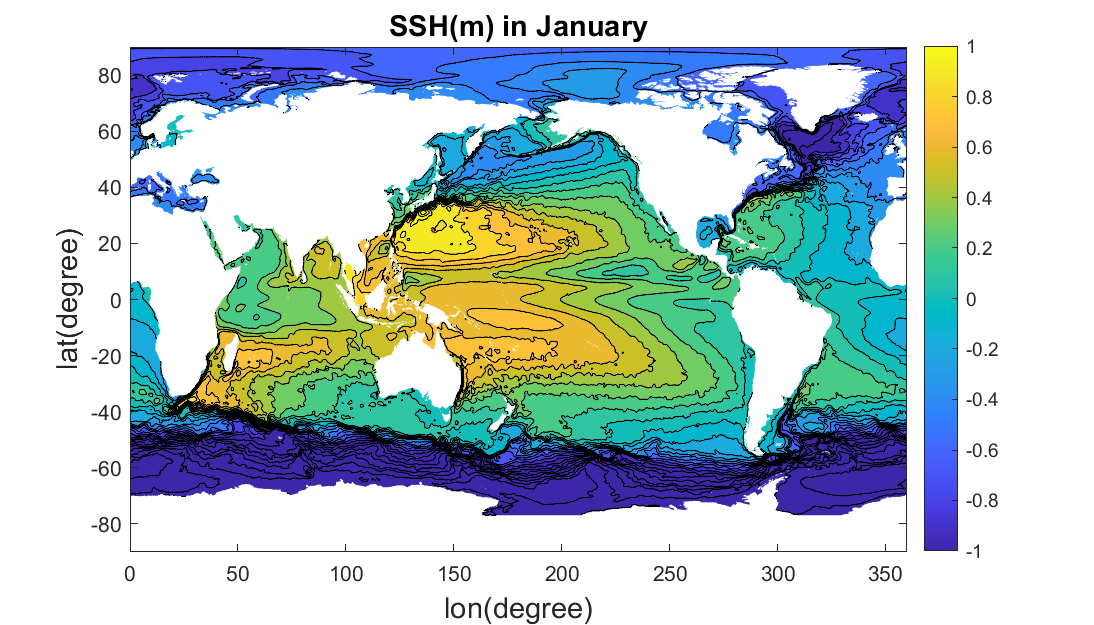
\includegraphics[width=1\textwidth]{Fig1a1.pdf}
	\caption{SSH distribution}
\end{figure}
In this report, we take care about the the average sea surface height of January. the Fig. (1) is my answer of \textbf{Problem 1}.\\

And  use a longitude convention in which the $x^\circ E$ is assigned as $x^\circ$. and the western longitudes are represented in a $0-360^\circ$ system such that $x^\circ W$ is converted to $(360-x)^\circ$. Thus that the Pacific can at the middle of the figure.\\

\textit{notice: this figure seems different from the picture showed in the Assignment. This is because the Figure in Assignment only color the SSH in the range $[-1, 1](m)$}
\newpage
%3
\section{Subtropical Rigion of N. Pacific}
\qquad And go focus on the region longitude $\in [120^\circ, 260^\circ]$, latitude $\in [5^\circ, 50^\circ]$. As the interior region of black frame in Fig. (2).
\begin{figure}[h]
 	\centering
	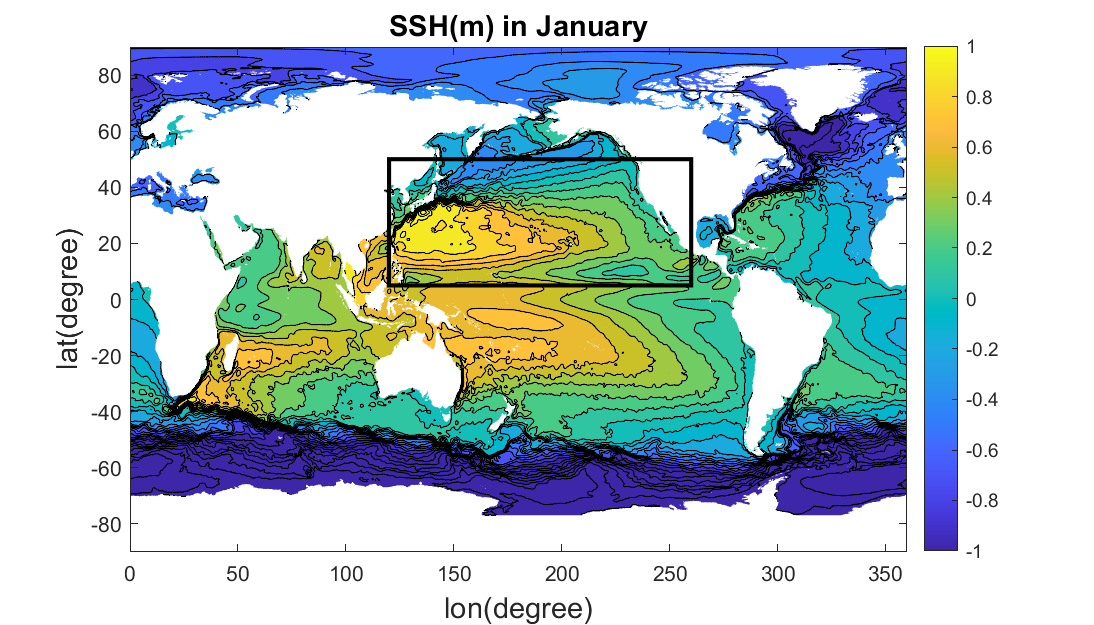
\includegraphics[width=0.8\textwidth]{Fig1a2.pdf}
	\caption{SSH distribution, the region in black frame is where we focus afterward}
\end{figure}
%3.1
\subsection{The Charactertistics of this region: SSH and velocity}
\begin{figure}[h]
 	\centering
	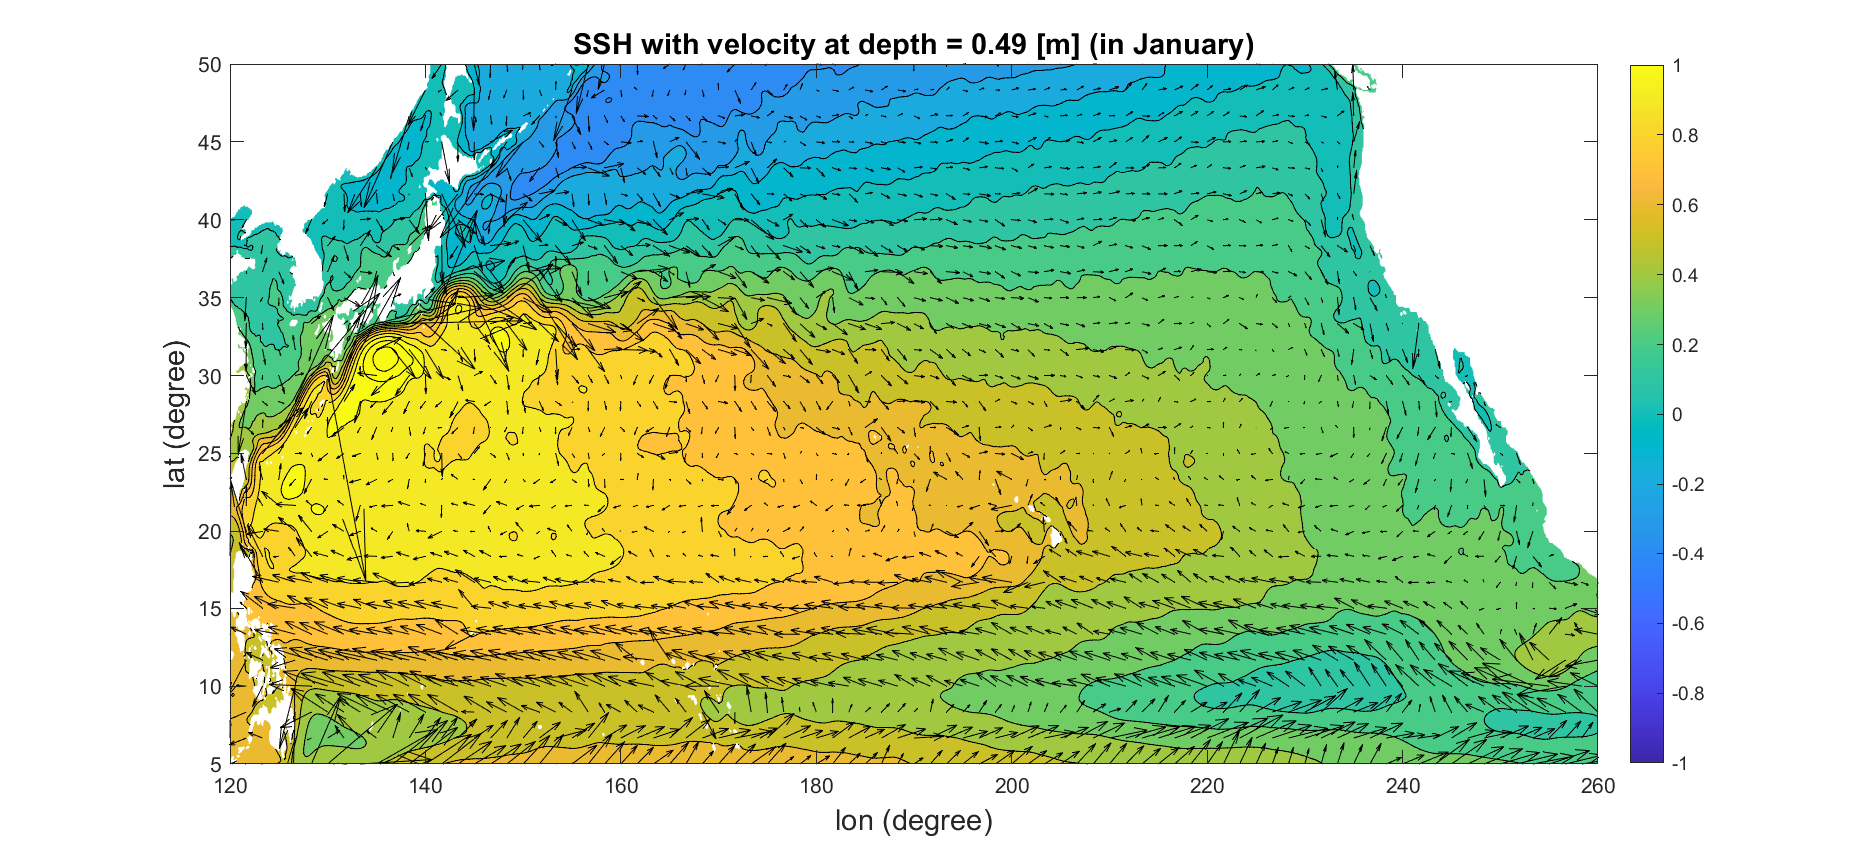
\includegraphics[width=0.9\textwidth]{Fig2a1.pdf}
	\caption{SSH with velocity at depth  = $0.4940 [m]$}
\end{figure}
In here, draw the SSH and the velocity in one picture as Fig.(3), in which I take the velocity data at the first vertical level at depth $h = 0.4904 [m]$ to plot velocity field. This is my answer of \textbf{Problem 2.(a)}
\newpage
%3.2
\subsection{The Subtropical gyre}
In here, throught analyze the velocity field in Fig.(3), I make a estimated region of subtropical gyre where framed by red rectangle as Fig.(4) shows: 
\begin{figure}[h]
 	\centering
	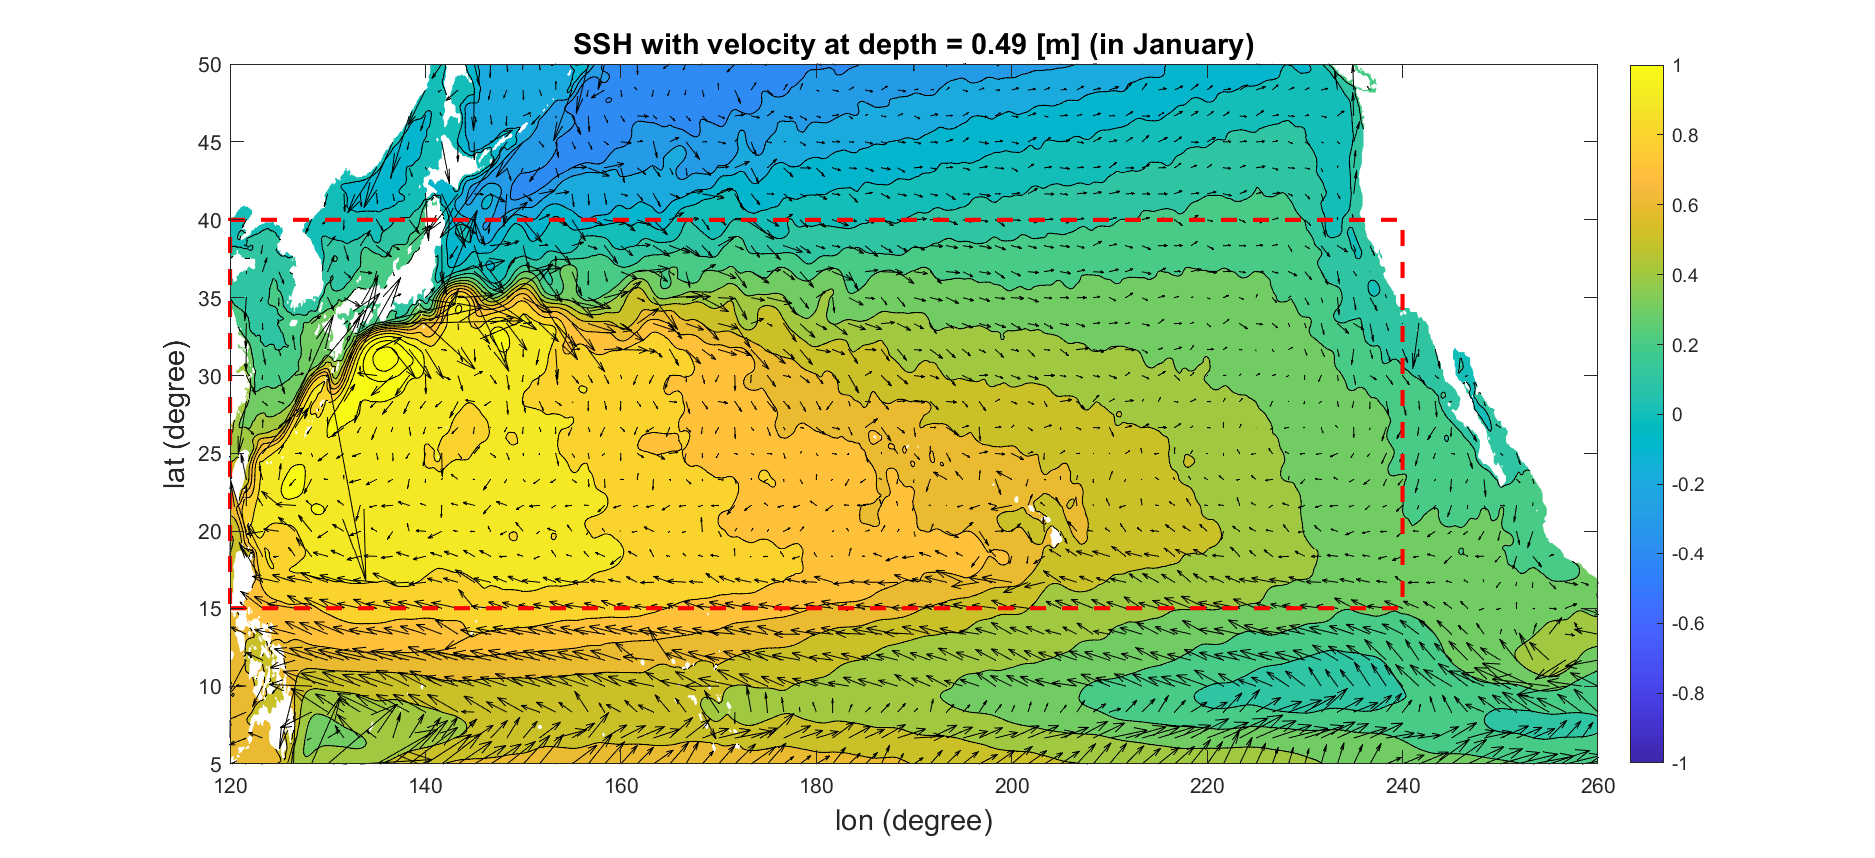
\includegraphics[width=0.9\textwidth]{Fig2b1.pdf}
	\caption{SSH with velocity at depth  = $0.4940 [m]$}
\end{figure}\\
Thus, I guessed the range of the subtropical gyre is longitude in $[120^\circ, 240^\circ]$ and latitude in $[15^\circ, 40^\circ]$ by the gyre's velocity direction (answer of \textbf{Problem 2.(b)(i)}).
\begin{figure}[h]
 	\centering
	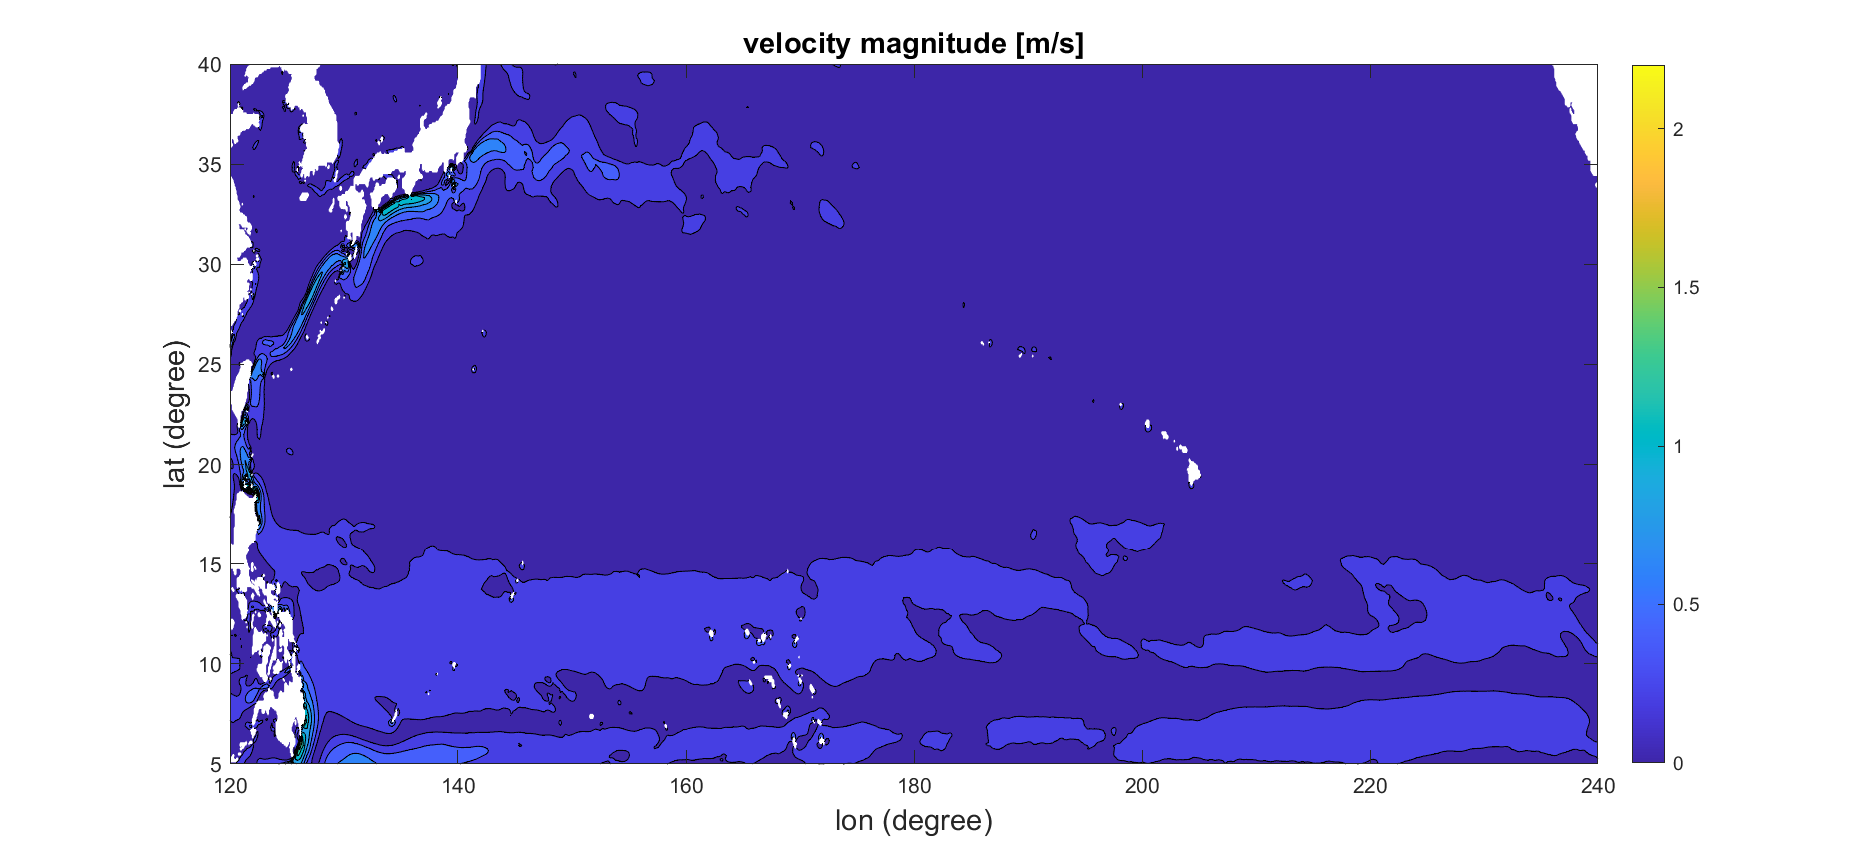
\includegraphics[width=0.9\textwidth]{Fig2b2.pdf}
	\caption{The velocity magnitude for gyre interior}
\end{figure}\\
Then compute the magnitude of velocity for gyre's interior, can draw a figure as Fig.(5) is also my answer of \textbf{Problem 2.(b)(ii)}. From which we can see that the magnitude in western is greater than other region. This is an manifestation of \textit{"Western Intensification"}. In this case, the western boundary current is \textbf{Kuroshio}. Let's go further.
%3.3
\subsection{Kuroshio}
First, I estimated the width of Kuroshio as following procedure:
\begin{enumerate}[(i)]
	\item Select the region near East China Sea (lon:$124^\circ$ to $131^\circ$, lat: $25^\circ$ to $31^\circ$) to analyze
	\item Estimate the span length of longitude $W_{lon}$ ($\vert{\vec{\textbf{u}}}\vert\ge 0.18[m/s]$) at lat: $28^\circ$
	\item Estimate the span length of longitude $H_{lat}$ ($\vert{\vec{\textbf{u}}}\vert\ge 0.18[m/s]$) at lon: $127.5^\circ$
	\item Compute the width $L_{Kuroshio}$ by using the properties of similar triangles
		\begin{equation}
			L_{Kuroshio} = W_{lon} \cdot \frac{H_{lat}}{\sqrt{W_{lon}^2+H_{lat}^2}}
		\end{equation}
\end{enumerate}

\begin{figure}[h]
 	\centering
	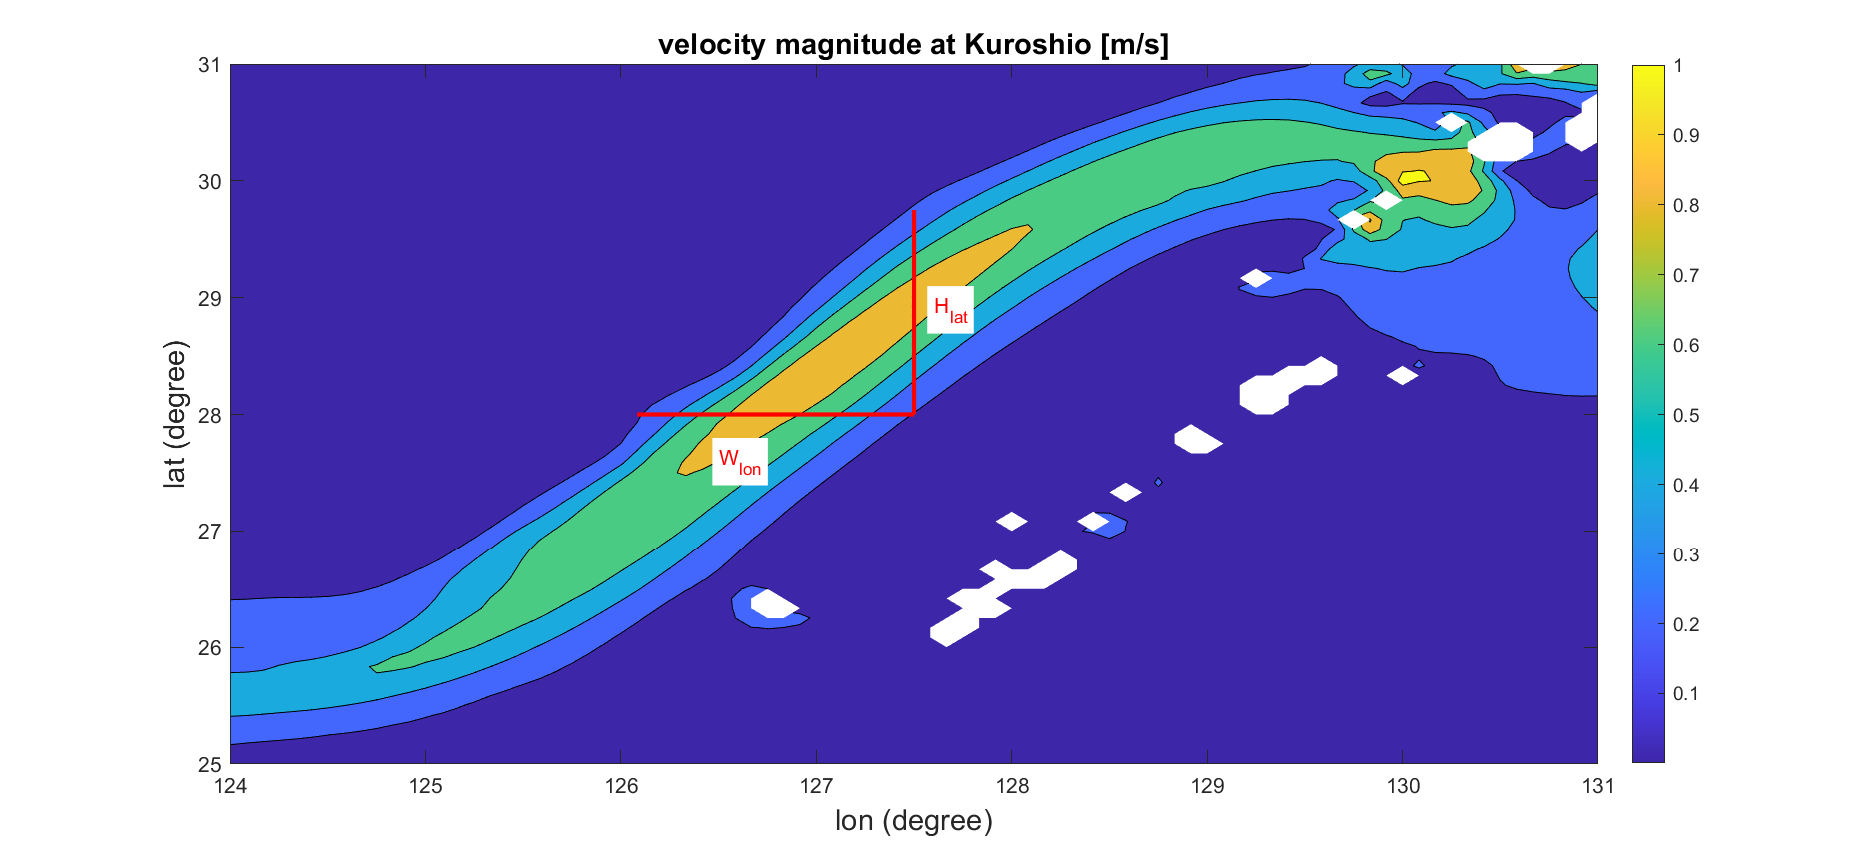
\includegraphics[width=1\textwidth]{Fig2b4.pdf}
	\caption{The velocity magnitude at Kuroshio (East China Sea),\\ white regions are islands}
\end{figure}
After computation, I have that: $W_{lon} = 139.09 [km], H_{lat} = 194.59 [km]$ as figure 6 shows, thus got the width of Kuroshio: $L_{Kuroshio} = 113.15 [km]$ which is my answer of \textbf{Problem 2.(b)(iii)}.\\

And estimated the characteristic velocity by average the velocity (of the data points in the red line of $W_{lon}$ Fig.(6) ) for the Kuroshio. Got the characteristic $U_{Kuroshio} = 0.56 [m/s]$. Which is also a part of \textbf{Problem 2.(b)(iii)}'s answer.\\

Last, compute the Rossby number of Kuroshio $Ro = \frac{U}{fL}$, let $f = 2\Omega \sin{(28^\circ)}$ in here, where $\Omega$ is the angular velocity of Earth's spin (地球自轉角速度). Got $Ro = 0.073$, (the answer of \textbf{Problem  2.(iv)}), which means that the movement of Kuroshio is influenced by Coriolis effect dominatly($Ro<1$), but the affect of ageostrophic effects cannot by entirely neglected (Rossby number around 0.1).
\newpage
%4
\section{Geostrophic velocity}
%4.1
\subsection{Geostrophic current and SSH}
\qquad Take a look at geostrophic velocity field. ($u_g, v_g$). Computed by Eq.(2)

\begin{equation}
\left\{
\begin{aligned}
	 u_g &= -\frac{g}{f} \frac{\partial \eta}{\partial y}\\
	 v_g &= \frac{g}{f} \frac{\partial \eta}{\partial x}
\end{aligned}
\right.
\end{equation}
In here, using $\Delta x = (a\cos{\phi}) \Delta \lambda$, $\Delta y = a\Delta \phi$, where $a$ is Earth's radius, and $\phi$, $\lambda$ are latitude and longitude in radian.\\
\begin{figure}[h]
 	\centering
	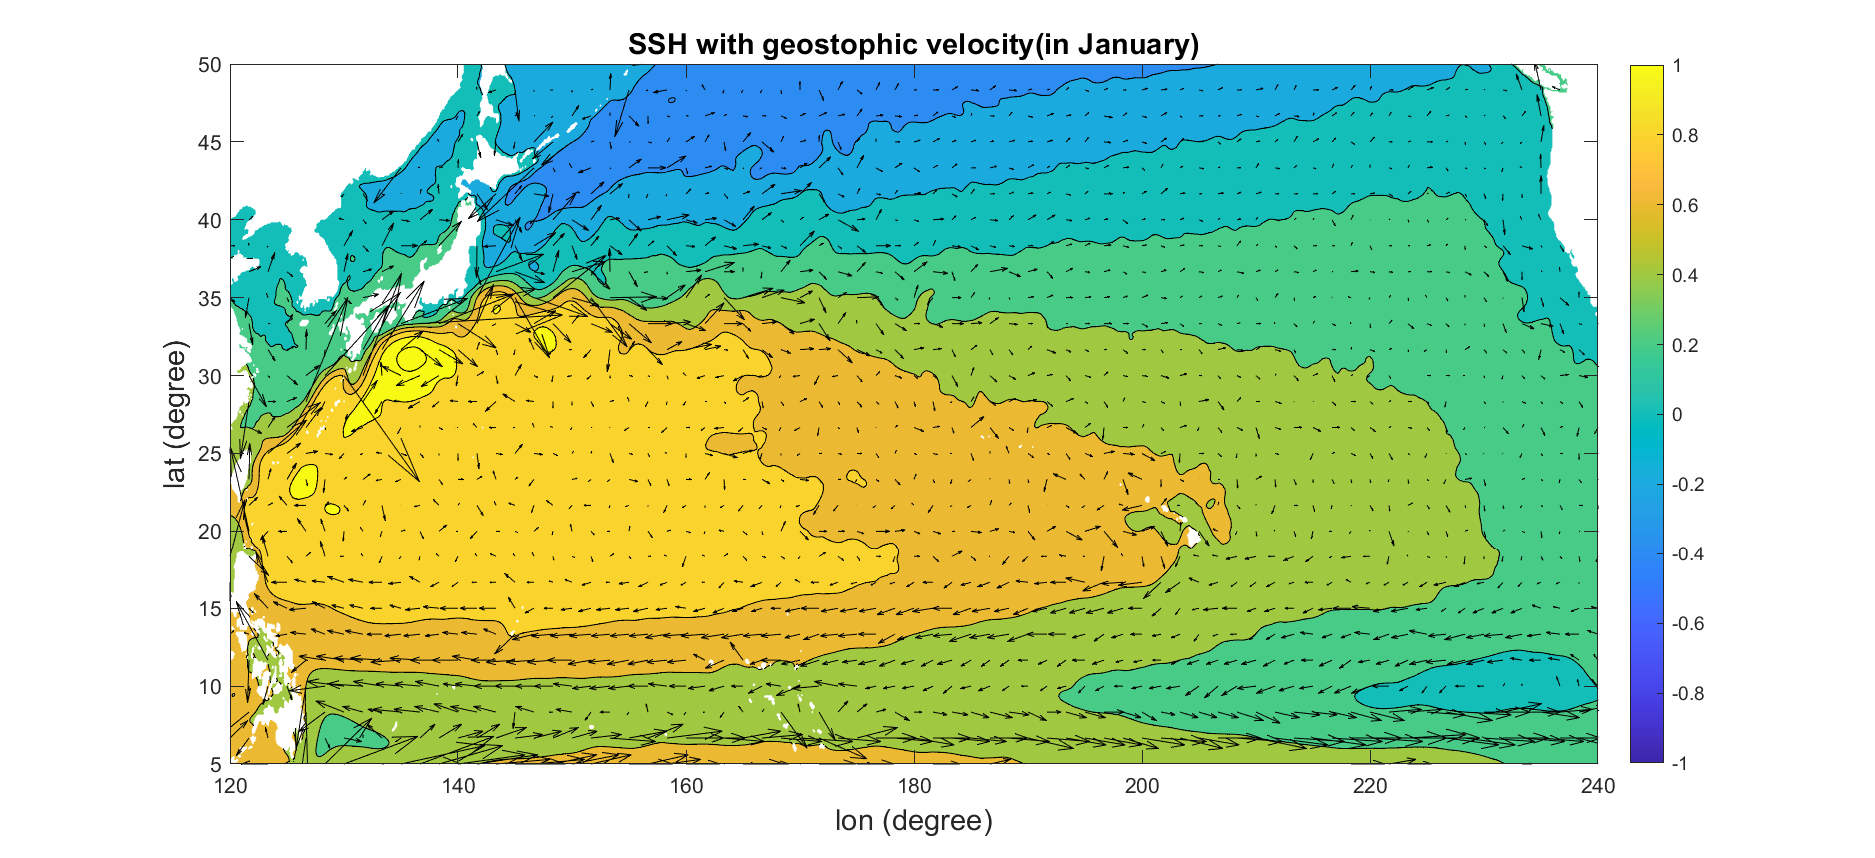
\includegraphics[width=1\textwidth]{Fig3a1.pdf}
	\caption{SSH with geostrophic velocity}
\end{figure}
From Fig.(7). The geostrophic velocity \textbf{is parallel} to the SSH contour, can be explain as:
\begin{equation}
\left\{
\begin{aligned}
	 &\text{direction of geostophic velocity} \qquad &\vec{v_1} \parallel(-\frac{\partial}{\partial y}, \frac{\partial}{\partial x})  \\
	 &\text{direction of SSH gradient}  \nabla \eta \qquad &\vec{v_2} \parallel (\frac{\partial}{\partial x}, \frac{\partial}{\partial y})
\end{aligned}
\right.
\end{equation}
Thus, the  inner product of these two vector is $0$, which also leads a conclusion that the two direction is perpendicular. On the other hand, the direction of geostophic vlocity is parallel to the SSH contour. Above are my answer of \textbf{Problem 3}\newpage
%4.2
\subsection{Geostrophic current and velocity field in different depth.}
\begin{figure}[h]
 	\centering
	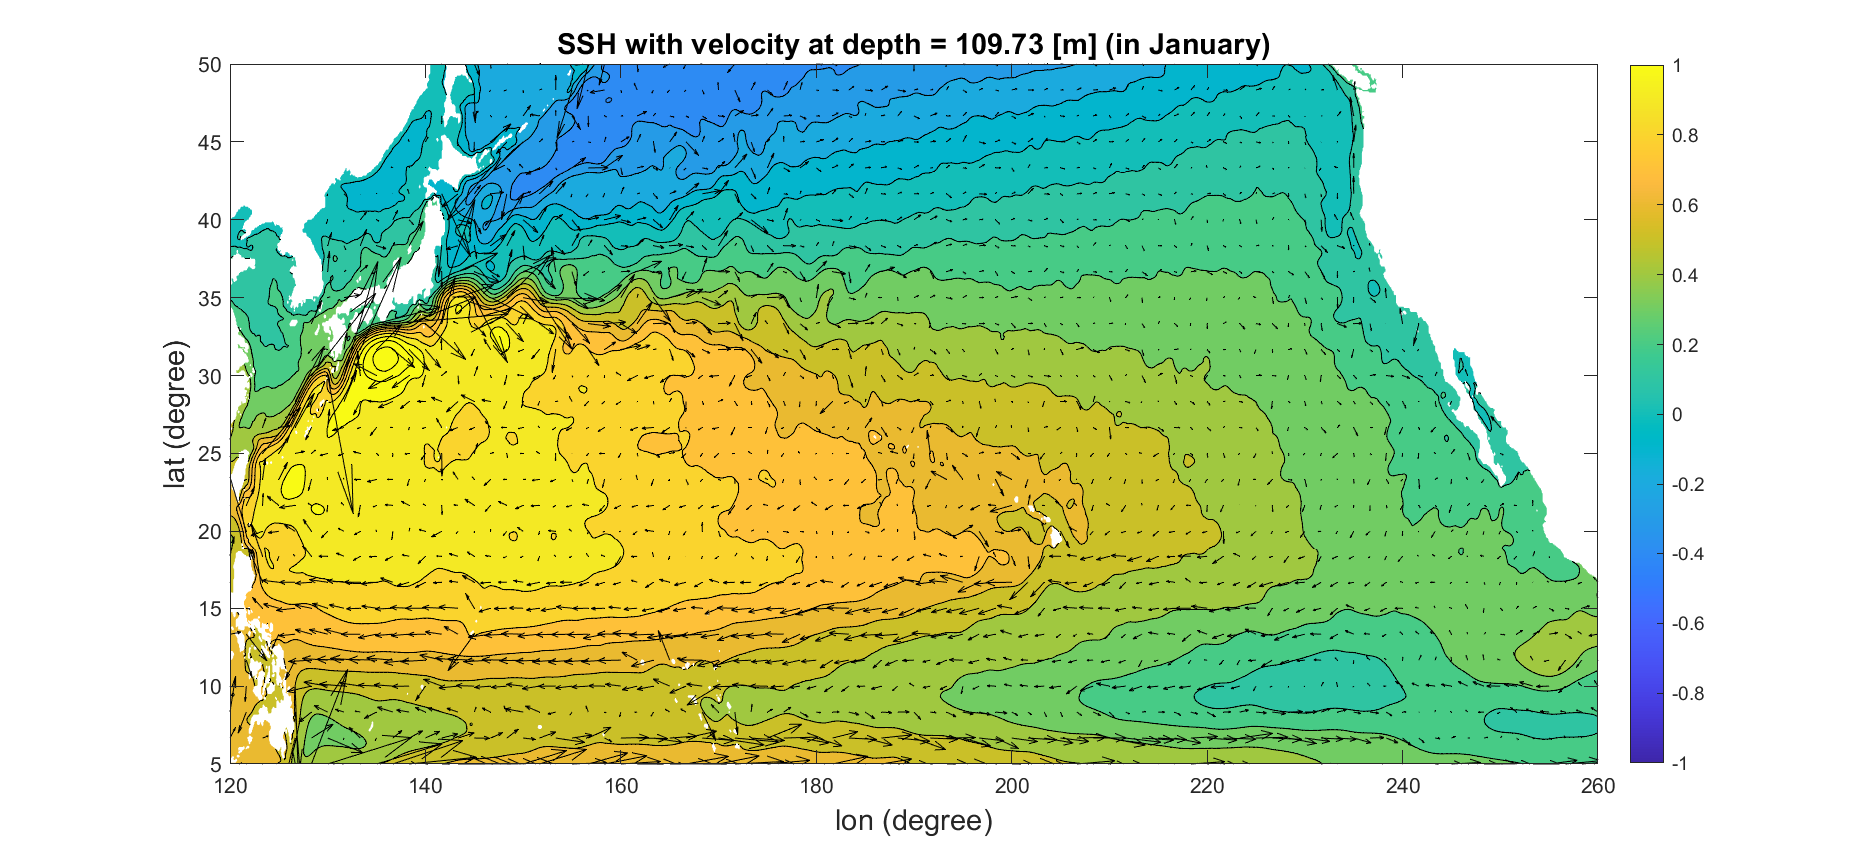
\includegraphics[width=1\textwidth]{Fig4a1.pdf}
	\caption{SSH with velocity at deep layer}
\end{figure}
Then I quantity differnce by calculate the sum of differece's square.
\begin{equation}
\left\{
\begin{aligned}
	 &\text{Surface layer}: \qquad &\sum \left[{(u_g-u_{surface})^2+(v_g-v_{surface})^2}\right] = 2.10\times 10^3\\
	 &\text{Depth layer}:\qquad &\sum \left[{(u_g-u_{depth})^2+(v_g-v_{depth})^2}\right] =6.75\times 10^2
\end{aligned}
\right.
\end{equation}
and we also can see that the velocity field at deep layer is much similar with geostophic velocity than surface layer. (By Fig.(3), (7), (8)). \\

The velocity at the ocean surface is affected by various external forces, including wind stress, waves, and tides. Notably, the influence of wind stress induces the \textit{"Ekman effect"}, which causes the flow to deviate from geostrophic balance and exhibit a spiral pattern with depth..
\newpage
%5
\section{Appendix: Program}
can downlowd figu
\begin{lstlisting}[
frame=single,
numbers=left,
style=Matlab-Pyglike
]
% Physical Oceanography Midterm report
% B11501037 Po-Tao, Lin
% This is the main program 
% And the program also upload to github
clear; close all;
%% Part 0 load data
filename = 'mercatorglorys12v1_gl12_mean_1993_2016_01.nc';
lon = ncread(filename, 'longitude');    % longitude (degree)
lat = ncread(filename, 'latitude');     % latitude (degree)
depth  = ncread(filename, 'depth');     % depth (m)
zos = ncread(filename, 'zos');          % SSH 
uo = ncread(filename, 'uo');            % eastward velocity
vo = ncread(filename, 'vo');            % north velocity

% sort the longitude by 180
lon360 = mod(lon, 360);
[lon360_sorted, idx] = sort(lon360);

zos_sorted = zos(idx, :);
uo_sorted = uo(idx, :,:);
vo_sorted = vo(idx, :,:);

%% Part 1
close all
figure('Position', [100, 100, 700, 400])

set(gcf, 'Color', 'white');
contourf(lon360_sorted, lat, zos_sorted.', 'Levelstep',0.1);
xlabel('lon(degree)','FontSize',14);
ylabel('lat(degree)','FontSize',14);
title('SSH(m) in January','FontSize',14);
axis([0 360 -90 90])
%ylim([-90, 90]);
colorbar;
clim([-1,1]);
exportgraphics(gcf, 'Fig1a1.pdf', 'ContentType', 'image');

%%% make similar picture with a black region
%lon = 120 to 260, lat = 5 to 50
hold on 
rectangle('Position', [120, 5, 140, 45], 'LineWidth',2);
hold off
exportgraphics(gcf, 'Fig1a2.pdf', 'ContentType', 'image');

%% Part 2-(i)
%onlyplot the region
[~, index_lon_w] = min(abs(lon360_sorted-120));
[~, index_lon_e] = min(abs(lon360_sorted-260));
[~, index_lat_s] = min(abs(lat-5));
[~, index_lat_n] = min(abs(lat-50));
figure('Position', [100, 100, 1200, 550])
set(gcf, 'Color', 'White');
lon_region = lon360_sorted(index_lon_w:index_lon_e);
lat_region = lat(index_lat_s:index_lat_n);
eta_region = squeeze(zos_sorted(index_lon_w:index_lon_e,index_lat_s:index_lat_n)).';
contourf(lon_region, lat_region, eta_region, 'Levelstep',0.1);
hold on
dx = 20; % take 1 data every 20 point
[lon_grid, lat_grid] = meshgrid(lon360_sorted(index_lon_w:dx:index_lon_e), lat(index_lat_s:dx:index_lat_n));
u_data = squeeze(uo_sorted(index_lon_w:dx:index_lon_e,index_lat_s:dx:index_lat_n,1)).';
v_data = squeeze(vo_sorted(index_lon_w:dx:index_lon_e,index_lat_s:dx:index_lat_n,1)).';
quiver(lon_grid, lat_grid, u_data, v_data,6,'k-')
colorbar
clim([-1,1]);
axis([120 260 5 50])
title(sprintf('SSH with velocity at depth = %.2f [m] (in January)', depth(1)),'FontSize',14);
xlabel('lon (degree)','FontSize',14);
ylabel('lat (degree)','FontSize',14);
exportgraphics(gcf, 'Fig2a1.pdf', 'ContentType', 'image');
%%% plot the estimated gyre
%%% the answer if problem 2.(i),estimated the range of gyre
rectangle('Position', [120, 15, 120, 25],'LineWidth',2,'LineStyle','--', 'EdgeColor','r');
exportgraphics(gcf, 'Fig2b1.pdf', 'ContentType', 'image');
hold off


%% Part 2-(ii) estimate the velocity magnitude of gyre
V_mag = sqrt(uo_sorted(:,:, 1).^2+vo_sorted(:,:, 1).^2);
[~, index_lon_gyre_w] = min(abs(lon360_sorted-120));
[~, index_lon_gyre_e] = min(abs(lon360_sorted-240));
[~, index_lat_gyre_s] = min(abs(lat-5));
[~, index_lat_gyre_n] = min(abs(lat-40));
figure('Position', [100, 100, 1200, 550])
set(gcf, 'Color', 'White');
contourf(lon360_sorted(index_lon_gyre_w:index_lon_gyre_e), ...
    lat(index_lat_gyre_s:index_lat_gyre_n),...
    squeeze(V_mag(index_lon_gyre_w:index_lon_gyre_e,index_lat_gyre_s:index_lat_gyre_n)).',...
    'Levelstep',0.2);
colorbar
title(sprintf('velocity magnitude [m/s]'),'FontSize',14);
xlabel('lon (degree)','FontSize',14);
ylabel('lat (degree)','FontSize',14);
exportgraphics(gcf, 'Fig2b2.pdf', 'ContentType', 'image');

%% Part 2-(iii) estimate the kuroshio
V_mag = sqrt(uo_sorted(:,:, 1).^2+vo_sorted(:,:, 1).^2);
[~, index_lon_kuroshio_w] = min(abs(lon360_sorted-124));
[~, index_lon_kuroshio_e] = min(abs(lon360_sorted-131));
[~, index_lat_kuroshio_s] = min(abs(lat-25));
[~, index_lat_kuroshio_n] = min(abs(lat-31));
%create the region of Kuroshio
lon_kuroshio = lon360_sorted(index_lon_kuroshio_w:index_lon_kuroshio_e);
lat_kuroshio = lat(index_lat_kuroshio_s:index_lat_kuroshio_n);
V_mag_kuroshio = V_mag(index_lon_kuroshio_w:index_lon_kuroshio_e,...
    index_lat_kuroshio_s:index_lat_kuroshio_n);

figure('Position', [100, 100, 1200, 550])
set(gcf, 'Color', 'White');
contourf(lon_kuroshio, lat_kuroshio, squeeze(V_mag_kuroshio).',...
    'Levelstep',0.2);
colorbar
title(sprintf('velocity magnitude at Kuroshio [m/s]'),'FontSize',14);
xlabel('lon (degree)','FontSize',14);
ylabel('lat (degree)','FontSize',14);
hold on
exportgraphics(gcf, 'Fig2b3.pdf', 'ContentType', 'image');

V_mag_threshold = 0.18;% determine the kuroshio velocity magnitude

% H_lat
target_lon = 127.5;
[~, ilon] = min(abs(lon_kuroshio-target_lon));
vsection = V_mag_kuroshio(ilon,:);
k_great_lat = find(vsection>V_mag_threshold); % velocity greater than 0.2 in lat
k_s = k_great_lat(1); k_n = k_great_lat(end); % latitude range
% W_lon
target_lat = 28;
[~, ilat] = min(abs(lat_kuroshio-target_lat));
usection = V_mag_kuroshio(:,ilat);
k_great_lon = find(usection>V_mag_threshold); % velocity greater than 0.2 in lon
k_w = k_great_lon(1); k_e = k_great_lon(end); % latitude range


line([lon_kuroshio(k_w), lon_kuroshio(k_e)], [lat_kuroshio(ilat), lat_kuroshio(ilat)],'Color','red','Linestyle','-','Linewidth', 2);
text(126.5, 27.6,'W_{lon}','Color','r','FontSize',10,'BackgroundColor','white')
line([lon_kuroshio(ilon), lon_kuroshio(ilon)], [lat_kuroshio(k_s), lat_kuroshio(k_n)],'Color','red','Linestyle','-','Linewidth',2);
text(127.6, 28.9,'H_{lat}','Color','r','FontSize',10,'BackgroundColor','white')
hold off
exportgraphics(gcf, 'Fig2b4.pdf', 'ContentType', 'image');

% estimate the chracteristic width
RE = 6371e3; %earth radius in [m]
W_lon = RE*cos(deg2rad(lat_kuroshio(ilat)))*(deg2rad(lon_kuroshio(k_e)-lon_kuroshio(k_w)));
H_lat = RE*(deg2rad(lat_kuroshio(k_n)-lat_kuroshio(k_s)));
L_kuroshio = W_lon*H_lat/sqrt(W_lon^2+H_lat^2); % width of Kuroshio
fprintf('W_lon = %.2f[km]\n', W_lon/1e3);
fprintf('H_lat = %.2f[km]\n', H_lat/1e3);
fprintf('The width of Kuroshio W_Kuroshio = %.2f [km]\n', L_kuroshio/1e3);

% estimate the characteristic velocity
U_kuroshio = mean(V_mag_kuroshio(ilon,k_great_lat));
fprintf('The characteristic velocity of Kuroshio is %.2f [m/s]\n', U_kuroshio);

% estimate the Rossby number
f_Kuroshio = 2*(2*pi/86400)*sin(deg2rad(lat_kuroshio(ilat))); %Coriolis frequency
RO_kuroshio = U_kuroshio/(f_Kuroshio*L_kuroshio);
fprintf('The Rossby number of Kuroshio is %.3f\n', RO_kuroshio);
%% Part 3 
g = 9.81; % gravitational accleration [m/s^2]
% using same range in Part 2.(i)
lon_sub = deg2rad(lon360_sorted(index_lon_w:index_lon_e));  
lat_sub = deg2rad(lat(index_lat_s:index_lat_n));  

[lon_grid, lat_grid] = meshgrid(lon_sub, lat_sub);  % M x N

eta = zos_sorted(index_lon_w:index_lon_e, index_lat_s:index_lat_n).';

omega = 2*pi/86400;
[dx,dy, deta_inx, deta_iny, f, ug, vg] = deal(zeros(size(eta)));
for i =1:size(eta,1)-1
    for j = 1:size(eta,2)-1
        dx(i,j) = RE*cos(lat_sub(i))*(lon_sub(j+1)-lon_sub(j));
        dy(i,j) = RE*(lat_sub(i+1)-lat_sub(i));
        deta_inx(i,j) = eta(i,j+1)-eta(i,j);
        deta_iny(i,j) = eta(i+1,j)-eta(i,j);
        f(i,j) = 2*omega*sin(lat_sub(i));
    end
end
for i =1:size(eta,1)-1
    for j = 1:size(eta,2)-1
        ug(i,j) = -g/f(i,j)*deta_iny(i,j)/dy(i,j);
        vg(i,j) = g/f(i,j)*deta_inx(i,j)/dx(i,j);
    end
end
ug_data = squeeze(ug(1:20:end,1:20:end));
vg_data = squeeze(vg(1:20:end,1:20:end));

figure('Position', [100, 100, 1200, 550])
set(gcf, 'Color', 'White');
contourf(lon360_sorted(index_lon_w:index_lon_e), lat(index_lat_s:index_lat_n),...
    eta,'LevelStep',0.2);
colorbar
clim([-1,1]);
hold on
quiver(lon360_sorted(index_lon_w:20:index_lon_e), lat(index_lat_s:20:index_lat_n), ug_data, vg_data,6,'k-')
axis([120,240,5,50])
title(sprintf('SSH with geostophic velocity(in January)'),'FontSize',14);
xlabel('lon (degree)','FontSize',14);
ylabel('lat (degree)','FontSize',14);
exportgraphics(gcf, 'Fig3a1.pdf', 'ContentType', 'image');
hold off
%% Part 4


[~, index_lon_w] = min(abs(lon360_sorted-120));
[~, index_lon_e] = min(abs(lon360_sorted-260));
[~, index_lat_s] = min(abs(lat-5));
[~, index_lat_n] = min(abs(lat-50));
figure('Position', [100, 100, 1200, 550])
set(gcf, 'Color', 'White');
lon_region = lon360_sorted(index_lon_w:index_lon_e);
lat_region = lat(index_lat_s:index_lat_n);
eta_region = squeeze(zos_sorted(index_lon_w:index_lon_e,index_lat_s:index_lat_n)).';
contourf(lon_region, lat_region, eta_region, 'Levelstep',0.1);
hold on
dx = 20; % take 1 data every 20 point
[lon_grid, lat_grid] = meshgrid(lon360_sorted(index_lon_w:dx:index_lon_e), lat(index_lat_s:dx:index_lat_n));

u_data_depth = squeeze(uo_sorted(index_lon_w:dx:index_lon_e,index_lat_s:dx:index_lat_n,23)).';
v_data_depth = squeeze(vo_sorted(index_lon_w:dx:index_lon_e,index_lat_s:dx:index_lat_n,23)).';
quiver(lon_grid, lat_grid, u_data_depth, v_data_depth,6,'k-')
colorbar
clim([-1,1]);
axis([120 260 5 50])
title(sprintf('SSH with velocity at depth = %.2f [m] (in January)', depth(23)),'FontSize',14);
xlabel('lon (degree)','FontSize',14);
ylabel('lat (degree)','FontSize',14);
exportgraphics(gcf, 'Fig4a1.pdf', 'ContentType', 'image');

figure
uo_surf_origin = uo_sorted(index_lon_w:index_lon_e,index_lat_s:index_lat_n,1).';
vo_surf_origin = vo_sorted(index_lon_w:index_lon_e,index_lat_s:index_lat_n,1).';
contour(lon360_sorted(index_lon_w:index_lon_e), lat(index_lat_s:index_lat_n), (ug-uo_surf_origin).^2+(vg-vo_surf_origin).^2);
colorbar
surfaceerror = nansum(nansum((ug-uo_surf_origin).^2)+sum((vg-vo_surf_origin).^2));
fprintf('the error of surface layer is %.2e\n', surfaceerror);
figure
uo_depth_origin = uo_sorted(index_lon_w:index_lon_e,index_lat_s:index_lat_n,23).';
vo_depth_origin = vo_sorted(index_lon_w:index_lon_e,index_lat_s:index_lat_n,23).';
contourf(lon360_sorted(index_lon_w:index_lon_e), lat(index_lat_s:index_lat_n),  (ug-uo_depth_origin).^2+(vg-vo_depth_origin).^2);
colorbar
deptherror = nansum(nansum((ug-uo_depth_origin).^2)+sum((vg-vo_depth_origin).^2));
fprintf('the error of depth layer is %.2e\n', deptherror);
\end{lstlisting}

\end{CJK*}
\end{document}
